\documentclass[11pt,spanish]{article}
\usepackage[utf8]{inputenc}
\usepackage{babel}
\usepackage{fullpage}
\usepackage{listings}
\usepackage{mathpazo}
\usepackage{enumitem}
\usepackage{courier}
\usepackage{xcolor}
\usepackage{textcomp}
\usepackage{amsmath}
\usepackage{amssymb}
\usepackage{tikz}
\usepackage{fancyhdr}
\usepackage{graphics}
\usepackage{array}

\newcommand{\titulo}{Certamen 1, sábado 10 de diciembre de 2011}
\newcommand{\cc}[1]{\hfil\texttt{#1}\hfil}
\newcommand{\pond}[1]{[{\small\textbf{#1\%}}]}

\hyphenation{dia-grama}

\pagestyle{fancy}
\lhead{%
  {\Large\bfseries Programación---\titulo} \\
  Nombre: \nombre\hfill
  Rol:    \rol
  \vspace{2ex}
}
\chead{}\rhead{}\lfoot{}\cfoot{}\rfoot{}
\renewcommand{\headrulewidth}{0pt}
\addtolength{\headheight}{7ex}
\headsep=4ex


\newcommand{\onelinerule}{\rule[2.3ex]{0pt}{0pt}}
\newcommand{\twolinerule}{\rule[6.2ex]{0pt}{0pt}}
\newcommand{\respuesta}{\framebox[\textwidth]{\twolinerule}}
\newcommand{\nombre}{%
  \begin{tikzpicture}[xscale=.4,yscale=.7]
    \draw (0, 0) rectangle (22, 1);
  \end{tikzpicture}%
}
%\newcommand{\rol}   {\framebox[0.3\textwidth]{\onelinerule}}
\newcommand{\rol}{%
  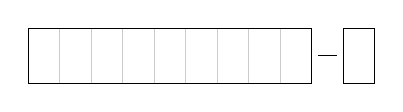
\begin{tikzpicture}[xscale=.4,yscale=.7]
    \draw[gray!40] ( 0, 0) grid      ( 9, 1);
    \draw          ( 0, 0) rectangle ( 9, 1);
    \draw          (10, 0) rectangle (11, 1);
    \draw (9 + .2, .5) -- (10 - .2, .5);
  \end{tikzpicture}%
}
\newcommand{\li}{\lstinline}
\providecommand{\pond}[1]{[{\small\textbf{#1\%}}]}

\lstdefinelanguage{py}{%
  classoffset=0,%
    morekeywords={%
      False,class,finally,is,return,None,continue,for,lambda,try,%
      True,def,from,nonlocal,while,and,del,global,not,with,print,%
      as,elif,if,or,yield,assert,else,import,pass,break,except,in,raise},%
    keywordstyle=\color{black!80}\bfseries,%
  classoffset=1,
    morekeywords={int,float,str,abs,len,raw_input,exit,range,min,max,%
      set,dict,tuple,list,bool,complex,round,sum,all,any,zip,map,filter,%
      sorted,reversed,dir,file,frozenset,open,%
      array,zeros,ones,arange,linspace,eye,diag,dot},
    keywordstyle=\color{black!50}\bfseries,%
  classoffset=0,%
  sensitive=true,%
  morecomment=[l]\#,%
  morestring=[b]',%
  morestring=[b]",%
  stringstyle=\em,%
}

\lstdefinelanguage{testcase}{%
  moredelim=[is][\bfseries]{`}{`},%
  backgroundcolor=\color{gray!20},%
}

\lstdefinelanguage{file}{%
  frame=single,%
}

\lstset{language=py}
\lstset{basicstyle=\ttfamily}
\lstset{columns=fixed}
\lstset{upquote=true}
\lstset{showstringspaces=false}
\lstset{rangeprefix=\#\ }
\lstset{includerangemarker=false}

\newlist{certamen}{enumerate}{1}
\setlist[certamen]{%
  label=\arabic*.,
  font=\LARGE\bfseries,%
  labelindent=-.5in,%
  leftmargin=0pt,%
  labelsep=1em%
}



\begin{document}

  \begin{enumerate}[font=\Large\bfseries]

    \item
      \pond{25}
      Indique qué es lo que imprimen los siguientes programas.

      \foreach \x in {1,2} {
        \noindent
        \begin{minipage}[b]{.5\textwidth}
          \lstinputlisting{p\x.py}
          \framebox[.8\textwidth]{\rule[10ex]{0pt}{0pt}}
          \vspace{0.4em}
        \end{minipage}
      }

      Rutee el siguiente programa
      e indique qué es lo que imprime.

      Cada vez que el valor de una variable cambie,
      ponga su valor en una nueva fila de la tabla.
      La tabla tiene filas de sobra.

      \begin{minipage}[T]{.5\textwidth}
        \lstinputlisting{ruteo.py}
        \framebox[.8\textwidth]{\rule[10ex]{0pt}{0pt}}
      \end{minipage}
      \begin{minipage}[t]{.4\textwidth}\centering
        \begin{tabular}{|*{4}{p{2.6em}|}}\hline
            \cc{s} & \cc{c} & \cc{i} & \cc{j} \\ \hline\hline
            &&& \\\hline &&& \\\hline &&& \\\hline &&& \\\hline &&& \\\hline
            &&& \\\hline &&& \\\hline &&& \\\hline &&& \\\hline &&& \\\hline
            &&& \\\hline &&& \\\hline &&& \\\hline &&& \\\hline &&& \\\hline
            &&& \\\hline &&& \\\hline &&& \\\hline &&& \\\hline &&& \\\hline
            &&& \\\hline &&& \\\hline &&& \\\hline &&& \\\hline &&& \\\hline
         \end{tabular}
      \end{minipage}

    \newpage
    \item
      \pond{25}
      Un edificio tiene 25 pisos de 8 departamentos cada uno.
      La dueña del edificio ha definido una estrategia
      para ponerle precio a cada departamento.

      \begin{minipage}[T]{.71\textwidth}
        El número que identifica cada departamento se divide en dos partes:
        los dos últimos dígitos indican en qué posición está
        (de acuerdo al diagrama),
        y los restantes indican el piso.
        Por ejemplo, el departamento 1105 está en el undécimo piso,
        en la posición 5.
        \\[.6ex]
        Los dos departamentos al extremo derecho del diagrama
        tienen vista al mar,
        y los dos del extremo izquierdo
        tienen vista al cerro.
      \end{minipage}
      \hspace{1em}
      \begin{minipage}[T]{.25\textwidth}
        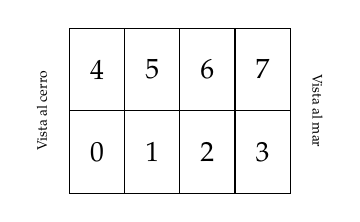
\begin{tikzpicture}[yscale=1.5, scale=.7]
          \draw (0, 0) grid (4, 2);
          \foreach\i in {0,...,3}
            \node at (+0.5 + \i, 0.5) {\i};
          \foreach\i in {4,...,7}
            \node at (-3.5 + \i, 1.5) {\i};
          \node[rotate=-90, font=\tiny] at ( 4.5, 1) {Vista al mar};
          \node[rotate=+90, font=\tiny] at (-0.5, 1) {Vista al cerro};
        \end{tikzpicture}
      \end{minipage}

      Todos los departamentos del primer piso valen 100,
      y todos los departamentos del último piso valen 400.

      Para los pisos intermedios,
      se ha fijado un precio base de 245;
      el precio de los departamentos con vista al mar se aumentará en 13\%,
      y el de los con vista al cerro se rebajará en 17\%.
      Los decimales se redondearán hacia abajo.

      Adicionalmente,
      se difundió el rumor de que el ídolo adolescente Justino Vivar
      habría alojado una noche en el departamento 807.
      Como hay un gran interés entre sus fanáticas
      por adquirir este departamento,
      la dueña ha decidido fijar su precio en 500.

      Escriba un programa que pregunte al comprador el número del departamento,
      y le entregue cuál es el precio de ese departamento.

    \newpage
    \item
      \pond{25}
      Un \emph{polinomio} de grado \(n\)
      es una función matemática que tiene la forma:
      \[
        p(x) =
        a_0     +
        a_1 x   +
        a_2 x^2 +
        a_3 x^3 +
        \cdots +
        a_n x^n.
      \]
      Los valores \(a_0, \ldots, a_n\)
      son los \emph{coeficientes} del polinomio,
      y \(x\) es la \emph{variable independiente}.

      \begin{minipage}[t]{.63\textwidth}
        Desarrolle un programa
        que evalúe un polinomio.
        \\[1ex]
        Primero,
        el usuario debe ingresar \(x\).
        A continuación,
        debe ingresar los coeficientes en orden.
        Para indicar que todos los coeficientes han sido ingresados,
        se debe escribir el texto \li!FIN!.
        Finalmente,
        el programa debe mostrar
        el valor de \(p(x)\).
        \\[1ex]
        El ejemplo de la derecha
        muestra cómo evaluar el polinomio
        \(p(x) = -7 - 3x^2 + 2x^3\) en \(x = 2.1\).
      \end{minipage}
      \hfill
      \begin{minipage}[t]{.26\textwidth}
        \lstinputlisting[language=testcase,frame=single]{caso-polinomio.txt}
      \end{minipage}

    \newpage
    \item
      \pond{25}
      El \emph{intercalao} es un juego muy popular
      entre los niños de la aldea de Pythópolis.

      El juego consiste en lanzar varias veces una moneda.
      En cada lanzamiento,
      el resultado puede ser cara (\li!C!) o sello (\li!S!).

      Un jugador gana cuando durante cuatro lanzamientos consecutivos
      aparecen caras y sellos intercalados
      (es decir, ningún resultado aparece dos veces seguidas),
      y pierde cuando un mismo resultado aparece
      cuatro veces seguidas.

      Escriba un programa que reciba como entrada
      los resultados de todos los lanzamientos
      hasta que termine el juego,
      y le indique al usuario si ganó o perdió.

      \begin{minipage}[t]{.26\textwidth}
        \lstinputlisting[language=testcase,frame=single,linerange=CASO\ 1-FIN\ CASO\ 1]{casos-intercalao.txt}
      \end{minipage}
      \hspace{1em}
      \begin{minipage}[t]{.26\textwidth}
        \lstinputlisting[language=testcase,frame=single,linerange=CASO\ 2-FIN\ CASO\ 2]{casos-intercalao.txt}
      \end{minipage}

  \end{enumerate}
\end{document}

